\section{向量的运算} \label{sec:vec-calc}

我们知道数量有加减乘除的四则运算, 以及乘方, 开方等运算.
那么向量有哪些运算呢?
虽然实际上对于向量可以定义各种各样的运算,
但我们引入向量是要在几何问题中去应用,
所以我们基本只关注有明确几何含义的向量运算.

\subsection{向量的线性运算}

线性运算包含加法运算和数乘运算, 是向量最本质的两种运算.

\subsubsection{加减法}

设向量$\vec{a}=(a_1,\dots,a_n),\vec{b}=(b_1,\dots,b_n)$.
$\vec{a}$和$\vec{b}$的加法记作$\vec{a}+\vec{b}$,
减法记作$\vec{a}-\vec{b}$, 计算方法为
\begin{align*}
  \vec{a}+\vec{b} & = (a_1+b_1,\dots,a_n+b_n), \\
  \vec{a}-\vec{b} & = (a_1-b_1,\dots,a_n-b_n). \\
\end{align*}

几何上, 向量的加法对应有向线段的首尾相接.
如图\ref{fig:vector-add},
将若干个向量对应的有向线段首尾相接,
起点和终点连线对应的向量就是这些向量的和.

\begin{figure}[htbp]
  \centering
  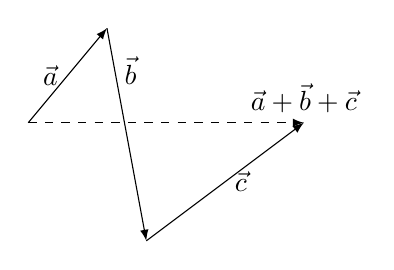
\begin{tikzpicture}
    \coordinate (A) at (0,0);
    \coordinate (B) at (1,1.2);
    \coordinate (C) at (1.5,-1.5);
    \coordinate (D) at (3.5,0);
    \begin{scope}[-latex]
      \draw (A) -- (B) node[left,pos=0.5] {$\vec{a}$};
      \draw (B) -- (C) node[right,pos=0.2] {$\vec{b}$};
      \draw (C) -- (D) node[right,pos=0.5] {$\vec{c}$};
      \draw[dashed] (A) -- (D) node[above]
      {$\vec{a}+\vec{b}+\vec{c}$};
    \end{scope}
  \end{tikzpicture}
  \caption{向量加法}
  \label{fig:vector-add}
\end{figure}

图\ref{fig:vector-sub}展示了向量减法的一个几何含义.
设点$A,B$对应的向量分别为$\vec{a},\vec{b}$,
那么有向线段$AB$对应的向量值为
$\vv{AB} = \vec{b} - \vec{a}$.

\begin{figure}[htbp]
  \centering
  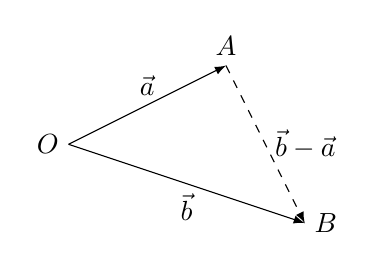
\begin{tikzpicture}
    \coordinate (A) at (2,1);
    \coordinate (B) at (3,-1);
    \node[left] at (0,0) {$O$};
    \node[above] at (A) {$A$};
    \node[right] at (B) {$B$};
    \begin{scope}[-latex]
      \draw (0,0) -- (A) node[above,pos=0.5] {$\vec{a}$};
      \draw (0,0) -- (B) node[below,pos=0.5] {$\vec{b}$};
      \draw[dashed] (A) -- (B)
      node[right,pos=0.5] {$\vec{b}-\vec{a}$};
    \end{scope}
  \end{tikzpicture}
  \caption{向量减法}
  \label{fig:vector-sub}
\end{figure}

\subsubsection{数乘}

向量$\vec{a}=(a_1,\dots,a_n)$和数值$\lambda$的乘法称为数乘,
沿用乘法的记法, 记作$\lambda\cdot\vec{a}$,
可以省略乘号, 记作$\lambda\vec{a}$. 计算方法为
\[
  \lambda\vec{a} = (\lambda a_1,\dots,\lambda a_n).
\]

向量数乘在几何上对应有向线段的伸缩.
对于向量$\vec{a}$和数值$\lambda$,
$\vec{a}$和$\lambda\vec{a}$是平行(共线)的, 并且
\begin{enumerate}[label=(\alph*)]
  \item $\lambda\vec{a}$的长度是$\vec{a}$的$|\lambda|$倍,
        即$|\lambda\vec{a}| = |\lambda| \cdot |\vec{a}|$;
  \item $\lambda>0$时, $\vec{a}$与$\lambda\vec{a}$方向相同;
        $\lambda<0$时, $\vec{a}$与$\lambda\vec{a}$方向相反.
\end{enumerate}

\begin{figure}[htbp]
  \centering
  \begin{tikzpicture}[scale=1.5]
    \node[dot,label={above:0}] {};
    \foreach \i/\k in {-2,-1/-,1/,2}
    \draw[-latex] (0,0) -- (\i,0) node[above] {$\k\vec{a}$};
  \end{tikzpicture}
  \caption{向量数乘}
  \label{fig:vector-mulnum}
\end{figure}

数乘与向量的平行(共线)有着紧密的联系:

\begin{theorem}\label{thm:vec-num-mul}
  对于向量$\vec{a}$和非零向量$\vec{b}$,
  $\vec{a}\parallel\vec{b}$
  当且仅当存在实数$\lambda\neq0$使得
  $\vec{a} = \lambda\vec{b}$.
\end{theorem}

\subsubsection{实例: 线性插值问题}

线性插值是向量线性运算的一个重要应用, 它讨论这样一个问题:
如何根据直线上的两个已知点的坐标, 计算直线上其他点的坐标?

\begin{theorem}[线性插值]
  设$n$维空间中有两个不重合的点$A=(a_1,\dots,a_n),B=(b_1,\dots,b_n)$.
  对于空间中的任一点$C=(c_1,\dots,c_n)$,
  点$C$在直线$AB$上, 当且仅当存在实数$a,b$使得$a+b=1$且
  \begin{align*}
    c_i = a \cdot a_i + b \cdot b_i,
    \quad (i=1,\dots,n).
  \end{align*}
  用向量运算表示即为$C = aA + bB$.
  特别地, 如果额外限制$0 \le a \le 1$
  (或者$0 \le b \le 1$),
  那么点$C$在线段$AB$上.
\end{theorem}

\begin{proof}
  我们需要证明``$C$在直线$AB$上''和``$C=aA+bB$''可以互相推导.
  \begin{enumerate}[label=(\alph*)]
    \item 如果点$C$在直线$AB$上, 那么$AB$与$AC$共线.
          根据向量数乘和向量共线的关联 (定理\ref{thm:vec-num-mul}),
          存在实数$\lambda$使得
          $\vv{AC}=\lambda\vv{AB}$. 于是有
          \begin{align*}
            C & = A + \vv{AC}                \\
              & = A + \lambda \vv{AB}        \\
              & = A + \lambda (B - A)        \\
              & = (1-\lambda) A + \lambda B.
          \end{align*}
          令$a=1-\lambda, b=\lambda$,
          则有$C=aA+bB, a+b=1$.
    \item 如果存在$a+b=1$使得$C=aA+bB$, 那么可以推导出
          \[\vv{AC} = b\vv{AB}.\]
          所以向量$\vv{AC},\vv{AB}$共线.
          考虑到$AC,AB$有公共的端点$A$,
          点$C$必然在直线$AB$上.
  \end{enumerate}
\end{proof}

\begin{figure}[htbp]
  \centering
  \begin{tikzpicture}
    \draw (3,2) coordinate (B)
    -- coordinate[pos=0.7] (C)
    (-1,3) coordinate (A);
    \coordinate (O) at (0,1);

    \begin{scope}[-latex]
      \draw (O) -- (A) node[left] {$A$};
      \draw (O) -- (B) node[right] {$B$};
      \draw (O) node[left] {$O$}
      -- (C) node[right,background] {$C = aA + bB$};
    \end{scope}
  \end{tikzpicture}
  \caption{线性插值 ($a=0.7$)}
  \label{fig:linear-interp}
\end{figure}

\subsection{二维向量的``乘积''}

向量的乘积是一个比较复杂的话题.
我们知道数量的乘法是非常直观的:
两个数相乘得到另一个数, 其含义是大小的缩放.
尽管单纯地定义一个向量``乘法''并不困难, 比如:

\begin{definition}[逐元素乘积]
  向量$\vec{a}=(a_1,\dots,a_n),\vec{b}=(b_1,\dots,b_n)$
  的\emph{逐元素乘积}的结果是一个向量, 记作$\vec{a}*\vec{b}$
  (乘号``$*$''不能省略),
  该向量的各个分量是$\vec{a},\vec{b}$的对应分量的乘积, 即
  \[
    \vec{a}*\vec{b} = (a_1b_1,\dots,a_nb_n).
  \]
\end{definition}

逐元素乘积是数量乘积的直接延伸, 看起来一切都很好.
只是有一个小小的问题: 我们定义一个运算是为了在实际场景中使用这个运算,
而在几何学, 向量用于描述有向线段等几何对象,
大小和方向是两个重要的几何属性,
但是在逐元素乘积中几乎无法讨论向量大小和方向的变化,
所以逐元素乘积的几何意义不大.

数学上主要讨论两种向量``乘积'': 内积和外积.
它们有类似于乘法的性质, 并且具有良好的几何意义.
由于一些难以说明的原因, 这一节只讨论\emph{二维向量}的内积和外积.

\begin{definition}[二维向量的内积]
  向量$\vec r_1=(x_1,y_1)$和$\vec r_2=(x_2,y_2)$
  的内积结果是一个数值, 记作$\vec r_1 \cdot \vec r_2$
  (乘号``$\cdot$''不能省略), 计算方法为
  \[
    \vec r_1 \cdot \vec r_2 = x_1x_2 + y_1y_2.
  \]
\end{definition}

\begin{definition}[二维向量的外积]
  向量$\vec r_1=(x_1,y_1)$和$\vec r_2=(x_2,y_2)$
  的外积结果是一个数值, 记作$\vec r_1 \times \vec r_2$
  (乘号``$\times$''不能省略), 计算方法为
  \[
    \vec r_1 \times \vec r_2 = x_1y_2 + x_2y_1.
  \]
\end{definition}

虽然它们的运算方法看起来有点怪,
但是它们有着明确的几何意义:

\begin{theorem}[内积与外积的几何意义]
  设$\vec r_1,\vec r_2$是两个二维向量, 它们的夹角为
  $\angle(\vec r_1,\vec r_2) = \theta$
  ($-180\degree < \theta \le 180\degree$),
  $\vec r_1$的长度为$|\vec r_1| = r_1$,
  $\vec r_2$的长度为$|\vec r_2| = r_2$.
  那么$\vec r_1,\vec r_2$的内积, 外积, 长度, 夹角之间有以下关系:
  \begin{align*}
    \vec r_1 \cdot \vec r_2  & = r_1 r_2 \cos\theta, \\
    \vec r_1 \times \vec r_2 & = r_1 r_2 \sin\theta.
  \end{align*}
\end{theorem}

限于篇幅, 我们在这里不进行证明, 这不会影响我们使用该定理.
如果你想知道怎么证明, 可以在网上搜索, 或者查看本教程的附录
\ref{sec:trig-proof}.

内积和外积之所以名字里有``积'',
是因为它们有类似乘积的\emph{分配律},
考虑到数乘, 我们把分配律稍作修改,
得到如下的内积和外积的线性性:
任取向量$\vec a_1,\vec a_2,\vec b$和实数$k_1,k_2$, 有
\begin{align*}
  (k_1\vec a_1 + k_2\vec a_2) \cdot \vec b
   & = k_1\,(\vec a_1 \cdot \vec b)
  + k_2\,(\vec a_2 \cdot \vec b),    \\
  \vec b \cdot (k_1\vec a_1 + k_2\vec a_2)
   & = k_1\,(\vec b \cdot \vec a_1)
  + k_2\,(\vec b \cdot \vec a_2),    \\
  (k_1\vec a_1 + k_2\vec a_2) \times \vec b
   & = k_1\,(\vec a_1 \times \vec b)
  + k_2\,(\vec a_2 \times \vec b),   \\
  \vec b \times (k_1\vec a_1 + k_2\vec a_2)
   & = k_1\,(\vec b \times \vec a_1)
  + k_2\,(\vec b \times \vec a_2),   \\
\end{align*}

除了分配律/线性性之外, 内积和外积还有一些独特的性质:
\begin{enumerate}[label=(\alph*)]
  \item 内积的交换律: $\vec a \cdot \vec b = \vec b \cdot \vec a$.
  \item 外积的反交换律: $\vec a\times\vec b = -\vec b\times\vec a$.
  \item $\vec a \times \vec a = 0$ 对任意二维向量$\vec a$成立.
\end{enumerate}

\subsubsection{内积与外积的应用}

内积可以用来表示向量长度. 设$\vec{r}=(x,y)$, 则有
$\vec{r}\cdot\vec{r} = x^2 + y^2 = |\vec{r}|^2$.

根据内积与夹角余弦值的联系, 我们可以用内积来
\begin{itemize}
  \item 判断垂直关系: 对于二维向量$\vec r_1,\vec r_2$,
        $\vec r_1 \bot \vec r_2$当且仅当
        $\vec r_1 \cdot \vec r_2 = 0$.
  \item 计算投影长度: 在图\ref{fig:vec-proj}中,
        已知线段$AB$的端点$A,B$和直线$CD$上的两点$C,D$,
        读者可以证明, $AB$在$CD$方向上的投影$A'B'$的长度为
        \begin{align}\label{eq:projection}
          |A'B'| = |AB|\cdot|\cos\angle(\vv{AB},\vv{CD})|
          = \dfrac{|\vv{AB}\cdot\vv{CD}|}{|CD|}.
        \end{align}
\end{itemize}

\begin{figure}[htbp]
  \centering
  \begin{tikzpicture}
    \draw (1,2) coordinate (A) node[left] {$A$}
    -- (2.5,1.5) coordinate (B) node[right] {$B$};
    \draw (0,0) coordinate (C) node[left] {$C$}
    -- (3.5,0.5) coordinate (D) node[right] {$D$};

    \begin{scope}[dashed]
      \draw (A) -- ($(C)!(A)!(D)$) node[below] {$A'$};
      \draw (B) -- ($(C)!(B)!(D)$) node[below] {$B'$};
    \end{scope}
  \end{tikzpicture}
  \caption{投影长度}
  \label{fig:vec-proj}
\end{figure}

由于外积与夹角正弦值的关系, 外积主要有以下应用:
\begin{itemize}
  \item 判断平行/共线关系: 对于二维向量$\vec r_1,\vec r_2$,
        $\vec r_1 \parallel \vec r_2$当且仅当
        $\vec r_1 \times \vec r_2 = 0$.
  \item 计算点到直线的距离: 在图\ref{fig:vec-dist}中,
        已知直线上的两点$A,B$, 对于平面上的一点$P$,
        可以证明点$P$到该直线的距离为
        \begin{align}\label{eq:distance}
          d = |AP| \cdot |\sin\angle(\vv{AB},\vv{AP})|
          = \dfrac{|\vv{AP}\times\vv{AB}|}{|AB|}.
        \end{align}
\end{itemize}

\begin{figure}[htbp]
  \centering
  \begin{tikzpicture}
    \draw (0,0) -- (4,0)
    coordinate[pos=0.2] (A)
    coordinate[pos=0.8] (B)
    coordinate[pos=0.6] (C);

    \draw (C) -- ($(C)!1.5cm!90:(B)$) coordinate (P)
    node[right,pos=0.5] {$d$};

    \node[dot,label={below:$A$}] at (A) {};
    \node[dot,label={below:$B$}] at (B) {};
    \node[right] at (P) {$P$};

    \draw[-latex,dashed] (A) -- (P);
  \end{tikzpicture}
  \caption{点到直线的距离}
  \label{fig:vec-dist}
\end{figure}

\subsection*{习题}

\begin{enumerate}
  \item 举例说明: 对于向量$\vec a,\vec b$,
        $|\vec a| + |\vec b|$与$|\vec a + \vec b|$不一定相等.
        试说明满足什么条件时二者是相等的.

  \item 已知平面上不重合的两点$A=(x_1,y_1),B=(x_2,y_2)$,
        求线段$AB$的两个三等分点的坐标.

  \item \comment{*}
        证明前文中用内积计算投影长度和用外积计算点到直线距离的方法
        (式\ref{eq:projection}, \ref{eq:distance}).

  \item \comment{镜面反射v2***}
        在之前的习题中我们讨论了子弹在版面边界的反弹.
        版面边界是水平线或竖直线, 所以计算起来是比较简单的.
        这一次我们考虑子弹在一个倾斜的反弹面 (直线) 上的反弹.

        \begin{figure}[htbp]
          \centering
          \begin{tikzpicture}[rotate=10,scale=1.2]
            \draw[line width=2pt] (0,-1.7) -- (0,1.7);
            \draw[->] (0,1.3) node[right] {$A$}
            -- +(-0.8,0) node[above] {$\theta,\vec n$};

            \draw[help lines] (150:3) -- (0,0) -- (-150:3);
            \draw[help lines,dashed] (0,0) -- (-30:2.5);
            \foreach \r in {2.3,1.3,0.3,-0.7}
            \node[dot] at (150:\r) {};
            \foreach \r in {0.7,1.7}
            \node[dot] at (-150:\r) {};
            \draw[->] (-2.2,1) -- +(-30:0.4);
            \draw[<-] (-2.2,-1) -- +(30:0.4);
            \draw[dashed]
            (-30:0.7) node[above] {$P$}
            -- (30:-0.7) node[left] {$P'$};

            \path (0,-1.5) node[left] {前侧} node[right] {后侧};
          \end{tikzpicture}
          \caption{镜面反射}
          \label{fig:rebound-v2}
        \end{figure}

        如图\ref{fig:rebound-v2},
        由反弹面上的一个点$A$, 以及一个垂直于反弹面的,
        指向前侧的单位向量$\vec n$, 可以确定该反弹面的位置.
        与版面边界反弹类似, 当子弹移动到反弹面的后侧时,
        我们需要修改子弹的速度, 朝向,
        并且计算子弹位置相对于反弹面的对称点.

        \begin{enumerate}[label=(\alph*)]
          \item 已知垂直于反弹面且指向前侧的方向角为$\theta$,
                请用$\theta$表示单位向量$\vec n$的值.
          \item 已知反弹面上的一点$A$以及垂直于反弹面且指向前侧的
                单位向量$\vec n$. 那么平面上的一点$P$满足什么条件时,
                可以判定$P$在反弹面的后侧?
          \item 若点$P$在反弹面的后侧, 设点$P'$是点$P$关于反弹面的对称点,
                求$PP'$的长度和点$P'$的坐标向量.
        \end{enumerate}
\end{enumerate}
